\documentclass[12pt]{extarticle}
%Some packages I commonly use.
\usepackage[english]{babel}
\usepackage{graphicx}
\usepackage{framed}
\usepackage[normalem]{ulem}
\usepackage{amsmath}
\usepackage{amsthm}
\usepackage{amssymb}
\usepackage{amsfonts}
\usepackage{enumerate}
\usepackage[utf8]{inputenc}
\usepackage[top=1 in,bottom=1in, left=1 in, right=1 in]{geometry}
\usepackage{xfrac}
\usepackage{hyperref}
\usepackage{listings}


\usepackage{array}
\newcolumntype{M}[1]{>{\centering\arraybackslash}m{#1}}
\newcolumntype{N}{@{}m{0pt}@{}}

%A bunch of definitions that make my life easier
\newcommand{\matlab}{{\sc Matlab} }
\newcommand{\cvec}[1]{{\mathbf #1}}
\newcommand{\rvec}[1]{\vec{\mathbf #1}}
\newcommand{\ihat}{\hat{\textbf{\i}}}
\newcommand{\jhat}{\hat{\textbf{\j}}}
\newcommand{\khat}{\hat{\textbf{k}}}
\newcommand{\minor}{{\rm minor}}
\newcommand{\trace}{{\rm trace}}
\newcommand{\spn}{{\rm Span}}
\newcommand{\rem}{{\rm rem}}
\newcommand{\ran}{{\rm range}}
\newcommand{\range}{{\rm range}}
\newcommand{\mdiv}{{\rm div}}
\newcommand{\proj}{{\rm proj}}
\newcommand{\R}{\mathbb{R}}
\newcommand{\N}{\mathbb{N}}
\newcommand{\Q}{\mathbb{Q}}
\newcommand{\Z}{\mathbb{Z}}
\newcommand{\<}{\langle}
\renewcommand{\>}{\rangle}
\renewcommand{\emptyset}{\varnothing}
\newcommand{\attn}[1]{\textbf{#1}}
\theoremstyle{definition}
\newtheorem{theorem}{Theorem}
\newtheorem{corollary}{Corollary}
\newtheorem*{definition}{Definition}
\newtheorem*{example}{Example}
\newtheorem*{note}{Note}
\newtheorem{exercise}{Exercise}
\newcommand{\bproof}{\bigskip {\bf Proof. }}
\newcommand{\eproof}{\hfill\qedsymbol}
\newcommand{\Disp}{\displaystyle}
\newcommand{\qe}{\hfill\(\bigtriangledown\)}
\setlength{\columnseprule}{1 pt}

\newcommand\Tstrut{\rule{0pt}{2.6ex}}       % "top" strut
\newcommand\Bstrut{\rule[-0.9ex]{0pt}{0pt}} % "bottom" strut
\newcommand{\TBstrut}{\Tstrut\Bstrut} % top&bottom struts


\newtheorem{problem}{Problem}
\newtheorem{solution}{Solution}


\title{Firedrake:  A complete package for solving partial differential equations using finite element methods}
\author{Justin Crum}
\date{May 19, 2020}
\begin{document}

\maketitle

\section{Introduction}

Firedrake is a python package solving partial differential equations through finite element methods.  To this end, the Firedrake developers have attempted to implement the major methods that have been covered in the Periodic Table of Finite Elements.

Firedrake works by interfacing with a few other packages.  Beyond just typical math packages for solving numerical problems like Eigen and petsc, Firedrake also makes use of packages UFL, TSFC, FIAT, and FInAT to get all the math done that it needs to do.

In this paper, we discuss the implementation of Serendipity and Trimmed Serendipity finite elements.  Serendipity elements had previously been implemented in two dimensions, but not in three dimensions entirely.  Trimmed Serendipity elements had not previously implemented in any dimension before this work began (within the Firedrake framework).

\section{Sections}

Probably need some words here about different things.  Like what are Serendipity and/or Trimmed Serendipity elements, previous work that was done, and possibly a bit about Firedrake.

\section{Work Done}

We have done the following:

\begin{enumerate}
    \item Implement Trimmed Serendipity elements in two dimensions.
    \item Tests have started on Trimmed Serendipity elements in two dimensions with promising results.
    \item In two dimensions, tests for Trimmed Serendipity have been conducted on both square/regular quad meshes as well as "arbitrary" quad meshes.  The test arbitrary quad mesh that we have made use of is a trapezoidal mesh, created by taking the configuration of the square mesh and moving select vertices up or down.
    \item Development of 3d Trimmed Serendipity elements is in progress.  
    \item Test on Trimmed Serendipity elements in three dimensions seem to indicate that this is still in the bug-testing phase.  Something is definitely either wrong with the PDE being solved (less likely, but possible) or wrong with the implementation (more likely).
    \item The 3d Trimmed Serendipity elements do in fact map basis functions to the proper entity (edge, face).  We do see the correct number of basis functions regardless of dimension.
\end{enumerate}

\section{What to do next?}

\begin{enumerate}
    \item We would like to continue tests on 2d Trimmed Serendipity.  This includes a couple of factors:
    \begin{enumerate}
        \item Check to make sure the correct functions are getting the correct entity (face/edge) assignment.  In two dimensions, this really only matters for edge assignment.
        \item Test 2d Trimmed Serendipity elements on an analytic test problem using numpy (somehow).  Goal here is to make sure that we can recreate polynomials exactly when we expect to.
        \item Check that the higher order portions of the 2d Trimmed Serendipity are implemented correctly--that basis functions are going to the right spot, that there are enough basis functions (this should be correct otherwise the code should break), and that the basis functions themselves are correctly implemented.
        \item Check sigma and divergence of sigma errors and make appropriate plots/charts/tables.  
    \end{enumerate}
    \item Continue bug testing on 3d Trimmed Serendipity elements.  This includes:
    \begin{enumerate}
        \item Check that basis functions are being implemented properly.
        \item Look closer at the PDE being used as a test PDE and make sure it is fitting for the type of problem we are doing.
        \item Test 3d Trimmed Serendipity on an analytic test problem and see if we recreate the polynomials we expect it to.
        \item If error is still bad....  Ask for a meeting with Andrew, Josh, and Rob all in the same zoom chat and figure out what else could be going wrong.
    \end{enumerate}
    \item Implement the 3d Serendipity elements for H(div) and H(curl).  These will be a little tricky to do, but will generally follow the same methodology used to implement the trimmed Serendipity elements.
    \item Continue remembering that H(div) is the column that is second to last and H(curl) is the column that comes second.  That is--H(div) elements mean that if I take a divergence of a vector element, I get a scalar element, whereas H(curl) elements mean that if I take a curl of a vector element, I get the next vector element.  
    \item Replace SminusE and SminusF in 2d fully with SminusCurl and SminusDiv fully.  Currently SminusDiv is in development.  The 2d portion should be able to replace SminusF entirely.  The 3d portion needs more work to see why the error is bad.  
\end{enumerate}

\section{Results}

Here we want to give some results from tests that we have done.  The following figures all depict a certain number of degrees of freedom vs error in the function and are based off a tides PDE problem where the mesh is a trapezoidal mesh.

Specifically, I have been running experiments on the tides PDE (described below) using RTC and S$^-$ elements on both square and trapezoidal meshes.  The RTC spaces get paired with DQ spaces from the same row of the periodic table.  The S$^-$ spaces get paired with DPC spaces from the same row of the table that Andrew has.  The figures below show the results of these simulations on the uniform square meshes.  

The code can be found at:\\


\noindent \url{https://github.com/Justincrum/MyFiredrakeWork/tree/master/TrimmedSerendipityTestCodes}\\


In the figures that follow, we should different types of degrees of freedom counts vs error.  The degrees of freedom that we count are either
\begin{enumerate}
    \item Shared degrees of freedom.  These are degrees of freedom that live on edges that are shared by more than one cell of the mesh.
    \item Total degrees of freedom.  This is just the total number of degrees of freedom in the mesh.
    \item Face degrees of freedom.  These are the degrees of freedom that are attached to a single face.  They are not shared by more than once cell of the mesh and do not live on the boundary.
\end{enumerate}


\begin{figure}
    \centering
    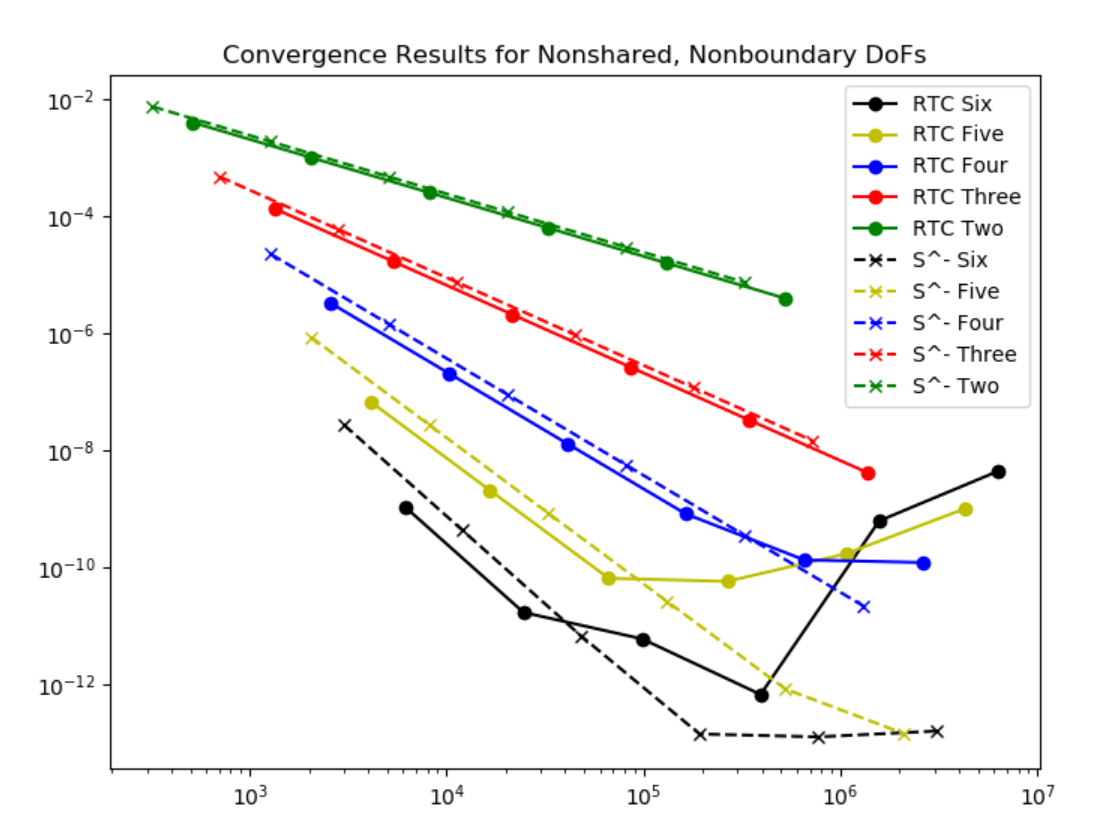
\includegraphics[width=10cm,height=10cm]{FaceDoFs.PNG}
    \caption{Showing the comparison of non-shared, non-boundary degrees of freedom vs error.}
    \label{fig:nonshared}
\end{figure}


\begin{figure}
    \centering
    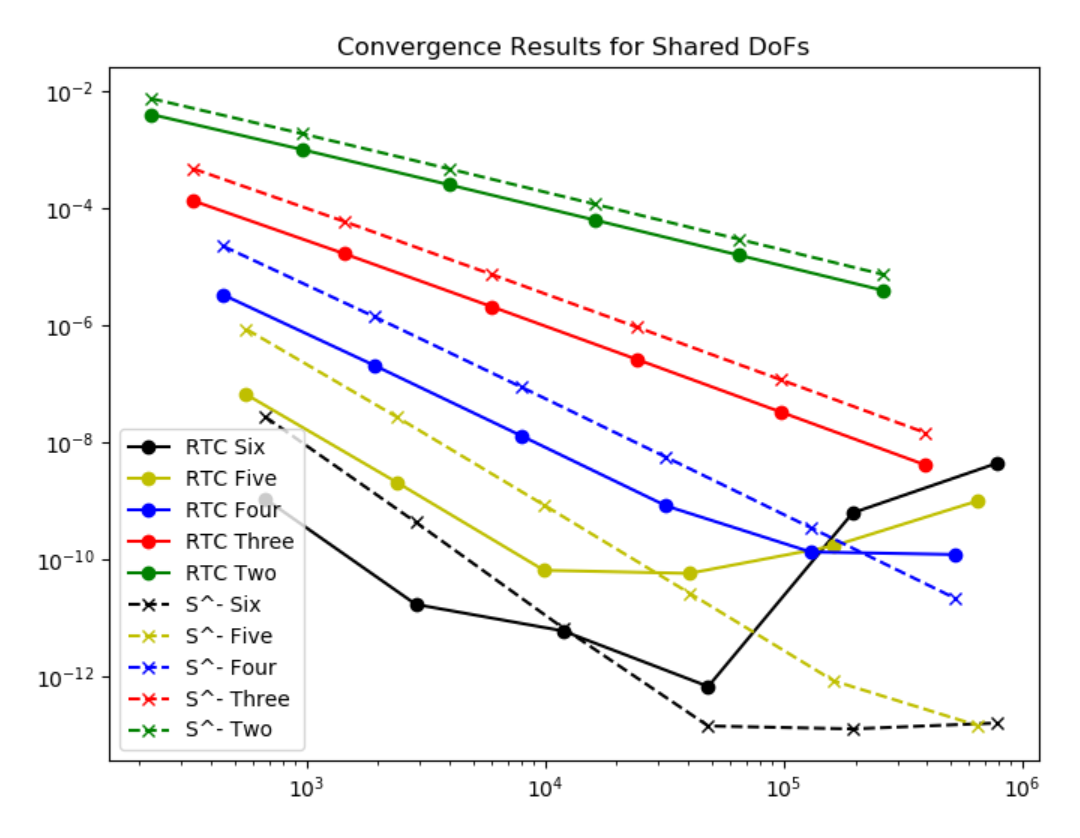
\includegraphics[width=10cm,height=10cm]{SharedDoFs.PNG}
    \caption{Showing the comparison of shared degrees of freedom vs error.}
    \label{fig:shared}
\end{figure}

\begin{figure}
    \centering
    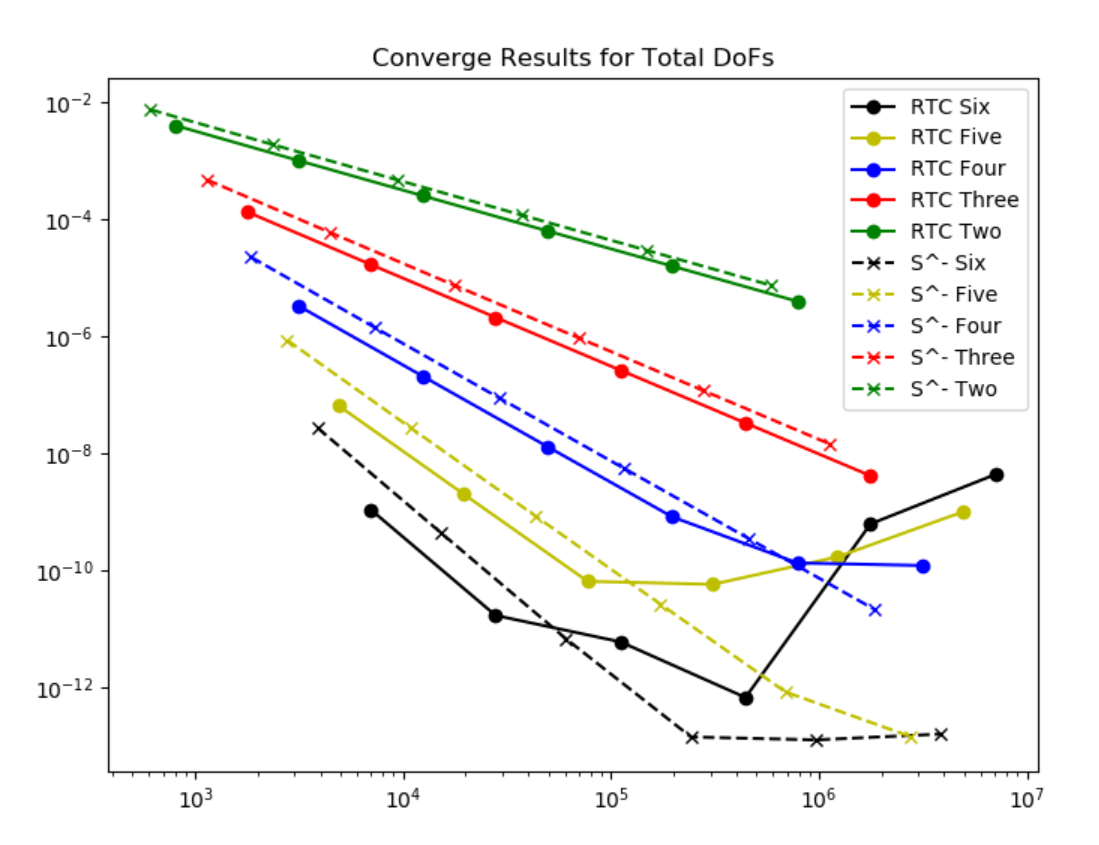
\includegraphics[width=10cm,height=10cm]{TotalDoFs.PNG}
    \caption{Comparison of total degrees of freedom vs error.}
    \label{fig:total}
\end{figure}

The experiments shown here done on uniform square meshes.  The convergences rates for trimmed Serendipity elements matches what we expect to see such that the convergence rate is equal to the polynomial degree that we choose.  The convergence rate for tensor product elements tends starts off converging to the proper value (again, the polynomial degree we choose), but then for higher degree polynomials we see a big burst in the error for higher mesh resolution.  

Current conjecture about this is that something about how many interior degrees of freedom the tensor elements produce is causing the solver issues at these higher mesh resolutions, but need a more experienced eye to help with drawing any conclusions.



\end{document}
